\documentclass[man]{apa6}
\title{ECE-5554 Computer Vision: Problem Set 0}
\author{Murat Ambarkutuk \\ murata@vt.edu}
\vfill
\affiliation{Mechanical Engineering Department,\\ Virginia Polytechnic Institute and State University}
\vfill
\note{\today \\ \LaTeX}
\usepackage{listings}
\usepackage{graphicx}
\usepackage{color} %red, green, blue, yellow, cyan, magenta, black, white
\definecolor{mygreen}{RGB}{28,172,0} % color values Red, Green, Blue
\definecolor{mylilas}{RGB}{170,55,241}

\shorttitle{Problem Set 0}
\leftheader{Even-Numbered Page Header}
\begin{document}
\maketitle

\lstset{language=Matlab,%
    %basicstyle=\color{red},
    breaklines=true,%
    morekeywords={matlab2tikz},
    keywordstyle=\color{blue},%
    morekeywords=[2]{1}, keywordstyle=[2]{\color{black}},
    identifierstyle=\color{black},%
    stringstyle=\color{mylilas},
    commentstyle=\color{mygreen},%
    showstringspaces=false,%without this there will be a symbol in the places where there is a space
    numbers=left,%
    numberstyle={\tiny \color{black}},% size of the numbers
    numbersep=12pt, % this defines how far the numbers are from the text
    emph=[1]{for,end,break},emphstyle=[1]\color{red}, %some words to emphasise
    %emph=[2]{word1,word2}, emphstyle=[2]{style},    
}

\section*{Matlab Code}

\section{Answer Sheet}
\subsection{Short answer problems}
	\begin{enumerate}
		\item Skipped.
		
		\item 
			\begin{enumerate}
				\item Creates a row vector containing random permutations of numbers between 1 and 1000.
				
				\item Line 1: Creates a matrix: \\
					\[ a= \left[ \begin{array}{ccc}
					1 & 2 & 3 \\
					4 & 5 & 6 \\
					7 & 8 & 9 \end{array} \right]\] 
					Line 2 assigns the second row of x to the variable b.
					$$ b = [4,5,6]$$

				\item Creates a matrix: \\
					\[ a= \left[ \begin{array}{ccc}
					1 & 2 & 3 \\
					4 & 5 & 6 \\
					7 & 8 & 9 \end{array} \right]\] 
					Line 2 assigns the all the values the variable b.
					\[ b= \left[ \begin{array}{ccc}
					1 & 2 & 3 \\
					4 & 5 & 6 \\
					7 & 8 & 9 \end{array} \right]\] 

				\item Line 1 creates the matrix f with the normally distributed random values. \\
					Line 2 sets another variable and fills it with the elements of f which are above 0.

				\item Line 1 sets a row vector  [1$\times10$] with zeros and adds 0.5 to each element of it.
					$$x= [0.5,0.5,0.5,0.5,0.5,0.5,0.5,0.5,0.5,0.5]$$
					Line 2 creates another row vector with the same size of vector x [1$\times10$], and multiplies each element of new row vector with 0.5. \\
					$$y= [0.5,0.5,0.5,0.5,0.5,0.5,0.5,0.5,0.5,0.5]$$
					Line 3 sums vector x and y and assigns the result to z.
					$$z = x + y$$
					$$z= [1,1,1,1,1,1,1,1,1,1]$$
					
				\item Line 1 creates a row vector [1$\times100$] which contains the sequence starting from 1 to 100 (inclusive).
					$$a= [1,2,3,4 \dots 98,99,100]$$
					Line 2 flips the vector and sets vector b with these values.
					$$a= [100,99,98,97 \dots 3,2,1]$$	
			\end{enumerate}
		
		\item The code is in PS0\_1-3.m file.
			\begin{enumerate}
			
				\item \lstinputlisting{diceTrials.m}
				
				\item \item \item \lstinputlisting{PS0_1_3.m}
			\end{enumerate}
		
		\item The code is in PS0Q1.m file.
		
			\begin{enumerate}
				\item Randomly generated intensity and the result of sort process.
					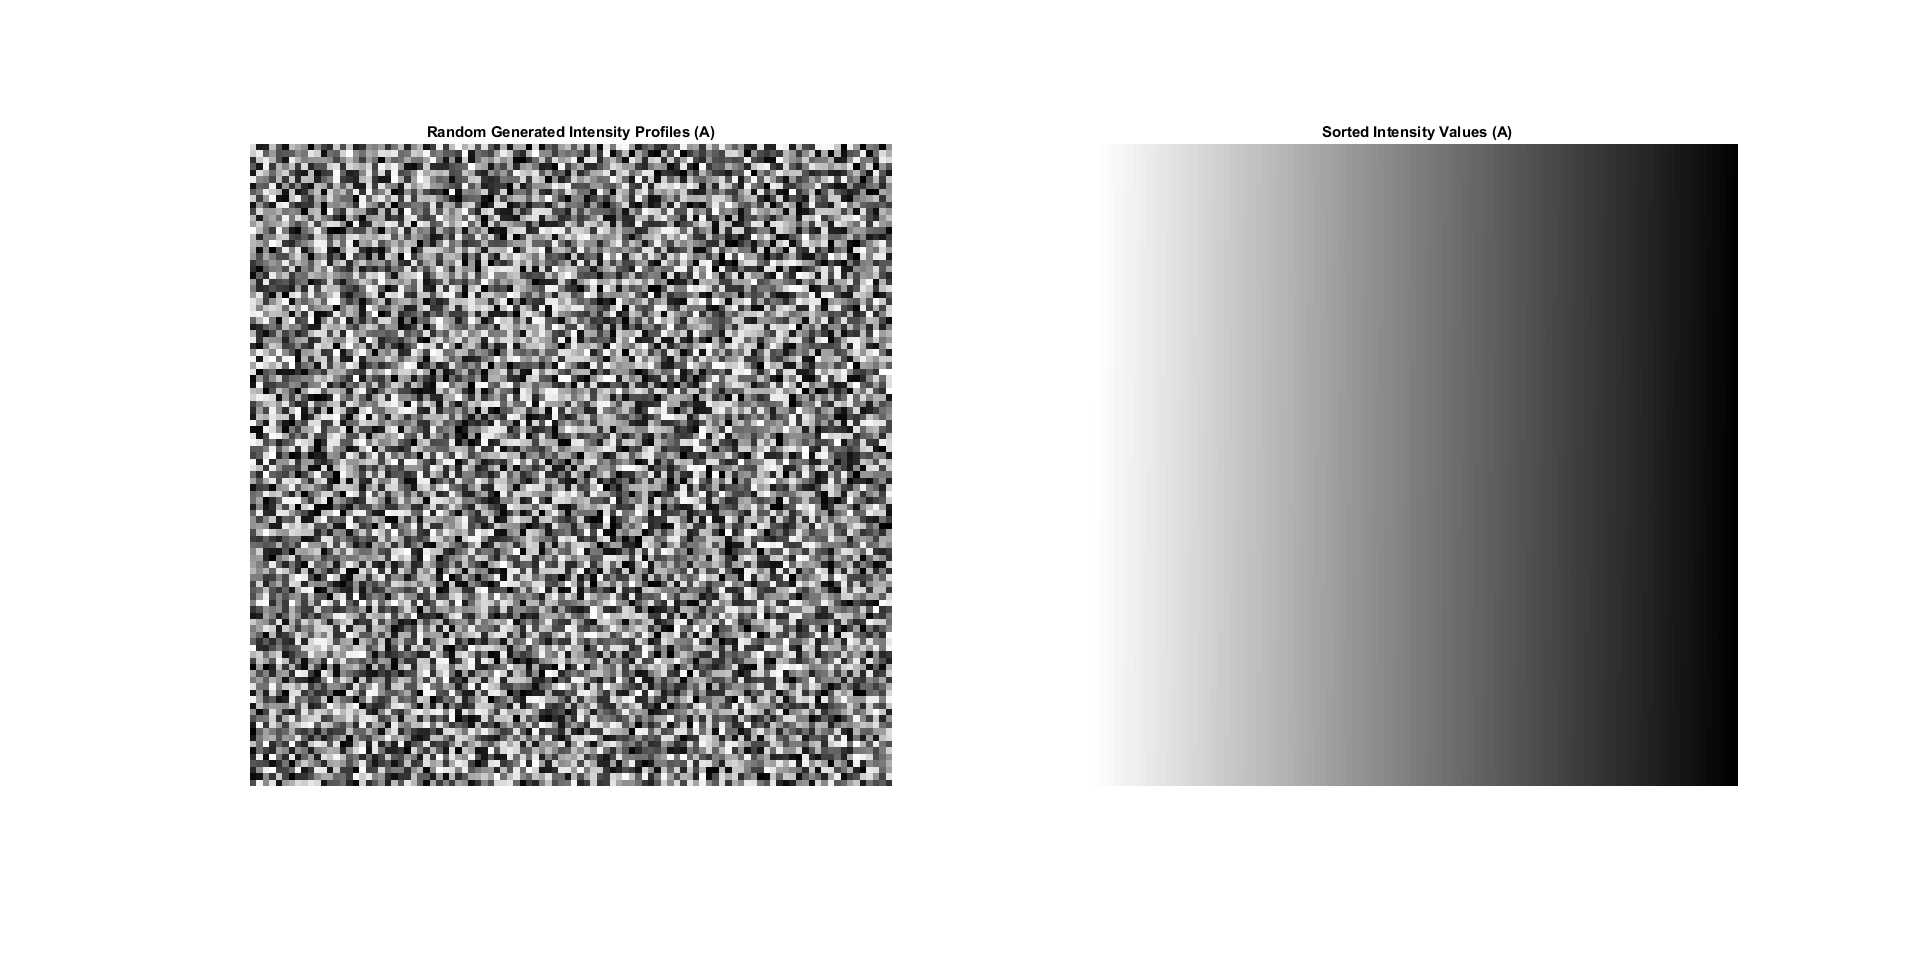
\includegraphics[width=\linewidth]{PS0-4.png}
			
				\item %###Insert plot###.
				
				\item %###Insert plot###. Please find the attached outputXPS0Q1.mat file.
				
				\item %###Insert plot###. Please find the attached outputYPS0Q1.mat file.
				
				\item %###Insert plot###. Please find the attached outputYPS0Q1.mat file.
				
				\lstinputlisting{PS0Q1.m}
			\end{enumerate}
		
	\end{enumerate}

\subsection{Short Programming Question}
	\begin{enumerate}
		\item
		\item
		\item
		\item
	\end{enumerate}
\end{document}
